\documentclass[aspectratio=169]{beamer}

\usetheme{default}

\usepackage[utf8]{inputenc}
\usepackage[russian]{babel}
\usepackage[OT1]{fontenc}
\usepackage{amsmath}
\usepackage{amsfonts}
\usepackage{amssymb}
\usepackage{graphicx}
\usepackage{etoolbox}
\usepackage{caption}
\usepackage{subcaption}
\captionsetup{compatibility=false}
\usepackage{pifont}
%\usepackage{subfigure}
\usepackage{xcolor}
\usepackage{framed}
\usepackage{empheq}
\usepackage[many]{tcolorbox}
\usepackage{multirow}
\usepackage{tikz}
\usepackage{listings}
\usepackage{tikz}

\definecolor{shadecolor}{cmyk}{0,0,0,1}

\lstset{
	backgroundcolor=\color{lightgray},
	commentstyle=\color{blue},
	frame=single
	breakatwhitespace, 
	language=python, 
	columns=fullflexible, 
	keepspaces, 
	breaklines, 
	tabsize=3, 
	showstringspaces=false, 
	extendedchars=true,
	numbers=left
}

\makeatletter

\setbeamercolor{title}{fg=white}
\setbeamercolor{frametitle}{fg=black}
\setbeamerfont*{title}{family=\sffamily,size=\LARGE}

\setbeamerfont{page number in head/foot}{size=\scriptsize}
\setbeamertemplate{footline}[frame number]
\let\otp\titlepage
\renewcommand{\titlepage}{\otp\addtocounter{framenumber}{-1}}

\setbeamertemplate{background canvas}{%
	\ifnumequal{\c@framenumber}{0}{%
		\vbox to \paperheight{\vfil\hbox to \paperwidth{\hfil
\includegraphics[height=\paperheight]{images/cover.png}\hfil}\vfil}
   }{%
      \ifnumequal{\c@framenumber}{\inserttotalframenumber}{
        \vbox to \paperheight{\vfil\hbox to \paperwidth{\hfil
\includegraphics[height=\paperheight]{images/back.png}\hfil}\vfil}
      }{%
         % Other frames
      }%
   }%
}

\makeatother

\beamertemplatenavigationsymbolsempty

\tcbset{highlight math style={enhanced,colframe=red,colback=white,arc=4pt,boxrule=1pt}}

\usetikzlibrary{shadings,shadows,shapes.arrows}

\newcommand*{\tikzarrow}[2]{%
  \tikz[
    baseline=(A.base),             % Set baseline to the baseline of node content
    font=\footnotesize\sffamily    % Set fontsize of the node content
  ]
  \node[
    single arrow,                  % Shape of the node
    single arrow head extend=5pt,  % Actual width of arrow head
    draw,                          % Draw the node shape
    inner sep=3pt,                 % Separation between node content and node shape
    top color=#1,               % Shading color on top of node
    bottom color=#1,               % Shading color on bottom of node
    % drop shadow                    % Draw a shadow
  ] (A) {#2};%
}

\newcommand{\tikzfancyarrow}[2][2cm]{\tikz[baseline=-0.5ex]\node [arrowstyle=#1] {#2};}
\newcommand*\rot{\rotatebox{90}}

\author{Николай Анохин}
\title{\newline \newline \newline Лекция 10 \\ Линейные модели \\ алгоритмическая перспектива}

\begin{document}

\begin{frame}[plain]
\titlepage
\end{frame}

\begin{frame}{План занятия}
\tableofcontents
\end{frame}


\begin{frame}{Постановка задачи}

{\bf Дано.} Признаковые описания $N$ объектов $\mathbf{x} = (x_1, \ldots, x_m) \in \mathcal{X}$, образующие тренировочный набор данных $X$, и значения целевой переменной $y = f(\mathbf{x}) \in \mathcal{Y}$ для каждого объекта из $X$. 

\vspace{1em}
{\bf Найти.} Для семейства параметрических функций 
\[
H = \{h(\mathbf{x, \mathbf{\theta}}) = y: \mathcal{X} \times \Theta \rightarrow \mathcal{Y}\},
\]
найти значение вектора параметров $\theta^*$, такое что $h^*(\mathbf{x}) = h(\mathbf{x}, \theta^*)$ наилучшим образом приближает целевую функцию.

\begin{eqnarray*}
Y & \in & \{C_1, C_2, \ldots, C_K\} \text{ -- задача классификации}  \\
Y & \in & [a, b] \subset \mathcal{R} \text{ -- задача регрессии}
\end{eqnarray*}

\end{frame}

\begin{frame}{Обобщенная линеная модель / GLM}

\[
y(\mathbf{x}, \mathbf{w}) \sim pdf\left[ f(\mathbf{w}^\top \phi(\mathbf{x})) \right],
\]
\begin{itemize}
\item $\phi_n(\mathbf{x})$ -- базисные функции
\item $f(a)$ -- функция активации
\item $pdf$ -- распределение из экспоненциального семейства
\end{itemize}

\end{frame}

% ============================================== %

\section{Линейные модели}

% ============================================== %

\begin{frame}{}

\begin{center}
\Large Обобщенные линейные модели

\vspace{1em}
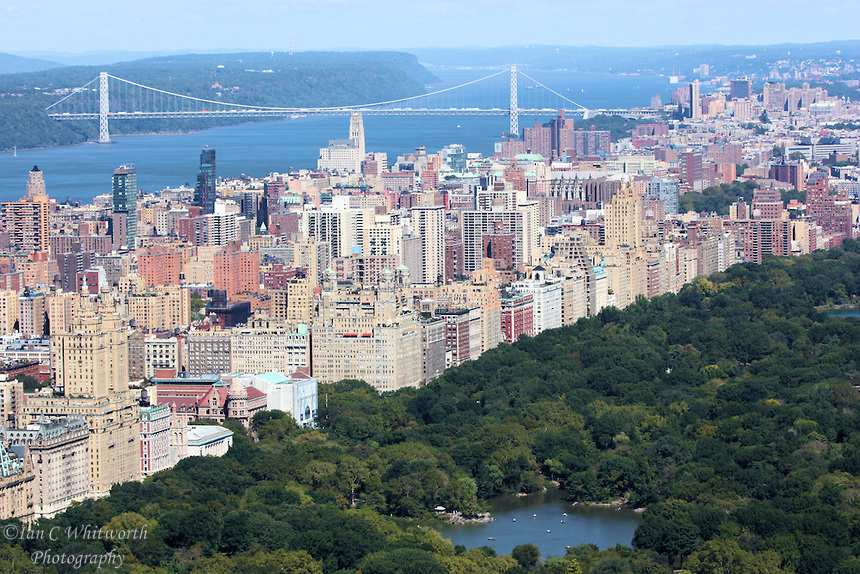
\includegraphics[height=0.7\textheight]{images/central_park.jpg}
\end{center}

\end{frame}

\begin{frame}{Линейные модели}

\begin{columns}[T]
    \begin{column}{.5\textwidth}
	Рассматривается случай 2 классов
	\vspace{0.3em} 
    
    Функция принятия решения
    \[
    y(\mathbf{x}) = \mathbf{w}^\top \mathbf{x} + w_0
    \]
    Регионы принятия решения
    \[
    R_1 = \{\mathbf{x}\,:\,y(\mathbf{x}) > 0\}
    \]
    \[
    R_2 = \{\mathbf{x}\,:\,y(\mathbf{x}) < 0\}
    \]
    Задача
    
    найти параметры модели $\mathbf{w}$, $w_0$
    \end{column}
       
    \begin{column}{.5\textwidth}
    \vspace{-0em}
	\begin{center}
   		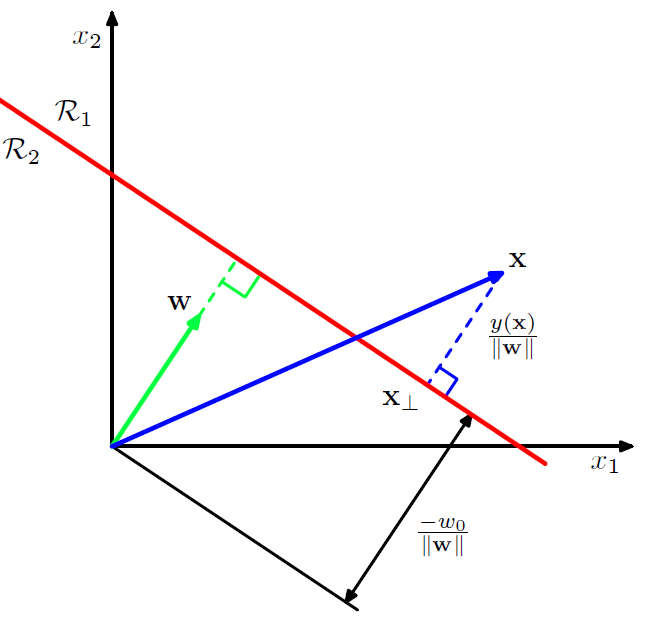
\includegraphics[scale=0.3]{images/linear.png}
    \end{center}
    \end{column}
  \end{columns}

\end{frame}

\begin{frame}{Линейные модели: наблюдения}

\begin{columns}[T]
    \begin{column}{.5\textwidth}
	Разделяющая поверхность
	\vspace{0.3em}
	\[
	\mathcal{D} = \{\mathbf x\,:\,\mathbf w^\top \mathbf x + w_0 = 0\}
	\]	
	
	\begin{enumerate}	
	\item $\mathbf{w}$ -- нормаль к $\mathcal{D}$
	
	\item $d = -\frac{w_0}{\|\mathbf{w}\|}$ -- расстояние от центра координат до $\mathcal{D}$
	
	\item $r(\mathbf{x}) = \frac{y(x)}{\|\mathbf{w}\|}$ -- расстояние от $\mathcal{D}$ до $\mathbf{x}$	
	\end{enumerate}
	
	Положим $x_0 \equiv 1$, получим модель
	\[
	y(\tilde{\mathbf{x}}) = \tilde{\mathbf w}^\top \tilde{\mathbf{x}}
	\] 
    
    \end{column}
       
    \begin{column}{.5\textwidth}
    \vspace{-0em}
	\begin{center}
   		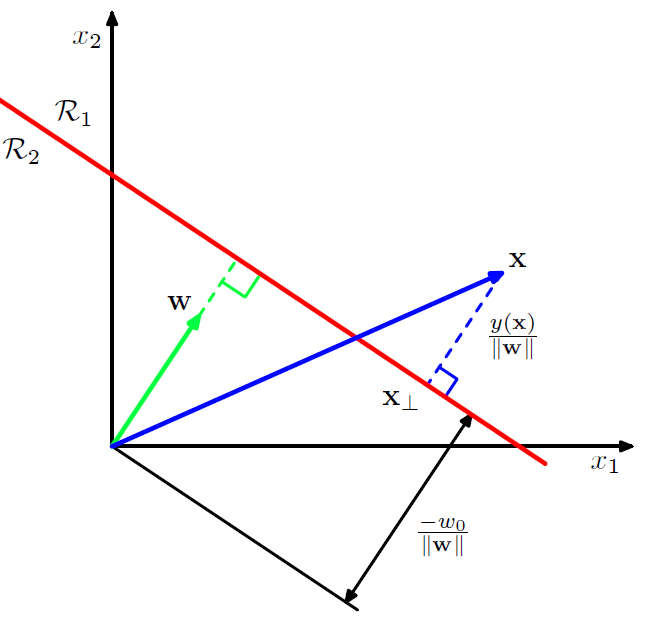
\includegraphics[scale=0.3]{images/linear.png}
    \end{center}
    \end{column}
  \end{columns}

\end{frame}

\begin{frame}{Мотивация}

\begin{center}
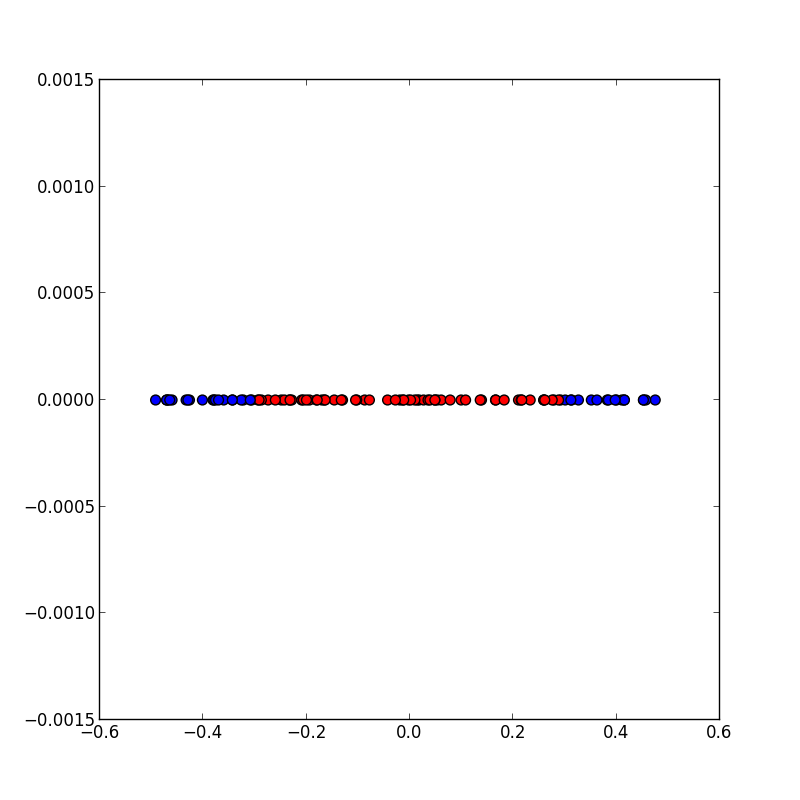
\includegraphics[scale=0.27]{images/pw1.png}
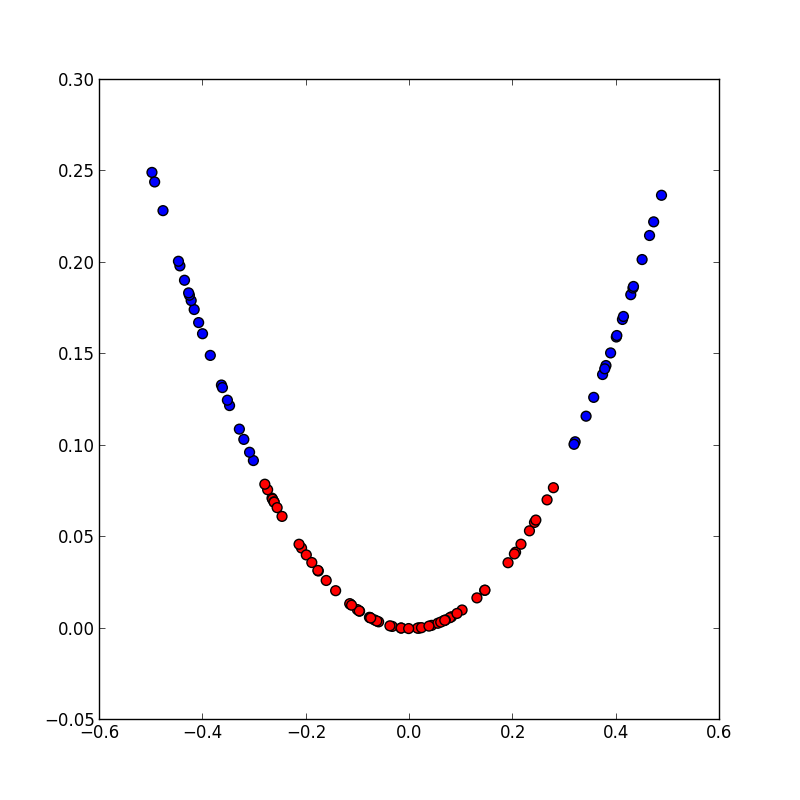
\includegraphics[scale=0.27]{images/pw2.png}
\end{center}

\end{frame}

\begin{frame}{Обобщенные линейные модели}

Линейная модель
\[
y(\mathbf{x}) = w_0 + \sum w_i x_i
\]
Квадратичная модель
\[
y(\mathbf{x}) = w_0 + \sum w_i x_i + \sum \sum w_{ij} x_i x_j
\]
Обобщенная линейная модель
\[
y(\mathbf{x}) = \sum w_i \phi_i(\mathbf{x})
\]

\end{frame}

\begin{frame}{Случай линейно разделимых классов}

Обобщенная линейная модель (внимание: переобозначения!)
\[
g(\mathbf{x}) = \sum w_i \phi_i(\mathbf{x}) \sim \mathbf{w}^T \mathbf{x}
\]
Дана обучающая выборка $D = (X, Y)$

\begin{center}
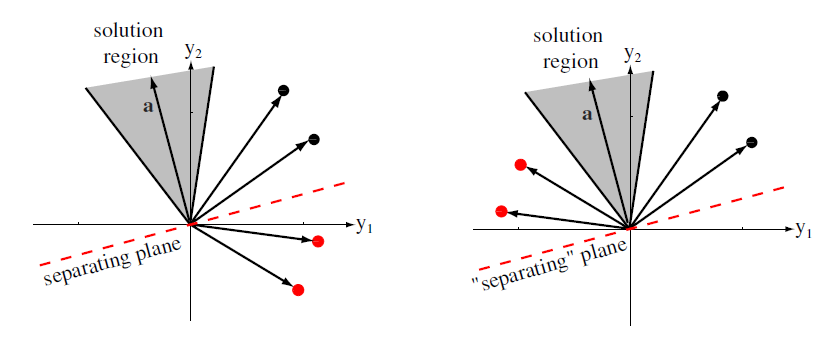
\includegraphics[scale=0.35]{images/optimzation.png}
\end{center}

\begin{exampleblock}{Идея}
Преобразовать объекты второго класса в обратные им и решать задачу оптимизации в области $\mathbf{w}^T \mathbf{x}_i > 0, \; \forall i$
\end{exampleblock}

\end{frame}

\begin{frame}{Задача оптимизации}

\begin{block}{Задача}
Минимизируем критерий $J(\mathbf{w})$ при условиях $\mathbf{w}^T \mathbf{x}_i > 0, \; \forall i$
\end{block}

Пусть $\mathcal{H}$ -- множество неправильно проклассифицированных объектов
\begin{itemize}
\item $J_e(\mathbf{w}) = \sum_{\mathbf{x} \in \mathcal{H}} 1$ 
\item $J_p(\mathbf{w}) = \sum_{\mathbf{x} \in \mathcal{H}} - \mathbf{w}^\top \mathbf{x}$ 
\item $J_q(\mathbf{w}) = \sum_{\mathbf{x} \in \mathcal{H}} (\mathbf{w}^\top \mathbf{x})^2$
\item $J_r(\mathbf{w}) = \sum_{\mathbf{x} \in \mathcal{H}} \frac{(\mathbf{w}^\top \mathbf{x} - b)^2}{\|\mathbf{x}\|}$
\end{itemize}
Улучшение: добавить отступы

\end{frame}

\begin{frame}{Логистическая регрессия}

функция правдоподобия (кросс-энтропия)
\[
J_c(\mathbf{w}) = - \sum_{n=1}^N {y_n \log \sigma(\mathbf{w}^T\mathbf{x}) + (1- y_n) \log (1 - \sigma(\mathbf{w}^T\mathbf{x}))} \rightarrow \min_{\mathbf{w}}
\]
Градиент
\[
\nabla J_c(\mathbf{w}) = \sum_{n=1}^N (p(y=1 | \phi_n) - y_n) \phi_n
\]
Гессиан
\[
\nabla^2 J_c(\mathbf{w}) = \sum_{n=1}^N p(y=1 | \phi_n) (1 - p(y=1 | \phi_n)) \phi_n \phi_n^T
\]

\end{frame}

\defverbatim[colored]\gd{%
\begin{lstlisting}[tabsize=4,basicstyle=\ttfamily]
function gd(grad, a0, epsilon):
	initialise eta(k)
	k = 0
	a = a0	 
	do:
		k = k + 1
		a = a - eta(k) grad(a)
	until eta(k) grad(a) < epsilon
	return a
\end{lstlisting}
}

\begin{frame}{Градиентный спуск}

	\gd

	\begin{center}
   		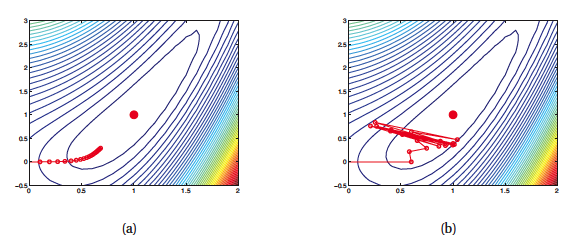
\includegraphics[scale=0.4]{images/gd.png}   		
    \end{center}
    
    Добавление момента: $\mathbf{a}_{k+1} = \mathbf{a}_k - \eta_k \nabla J (\mathbf{a}_k) + \mu_k (\mathbf{a}_{k} - \mathbf{a}_{k-1})$

\end{frame}

\defverbatim[colored]\newton{%
\begin{lstlisting}[tabsize=4,basicstyle=\ttfamily,basicstyle=\small]
function newton(grad, hessian, a0, epsilon):
	initialise eta(k)
	k = 0
	a = a0	 
	do:
		k = k + 1
		g = grad(a)
		H = hessian(a)
		d = solve(H * d = -g) # find d = - inv(H) * g
		a = a + eta(k) d
	until convergence
	return a
\end{lstlisting}
}

\begin{frame}{Метод Ньютона}

\begin{small}
\[
J(\mathbf{a}) \approx J(\mathbf{a}_k) + \nabla J(\mathbf{a}_k)^T (\mathbf{a} - \mathbf{a}_k) + \frac 1 2 (\mathbf{a} - \mathbf{a}_k)^T \nabla^2 J(\mathbf{a}_k) (\mathbf{a} - \mathbf{a}_k) \rightarrow \min_{\mathbf{a}}
\]
\[
\mathbf{a} = \mathbf{a}_k - \nabla^2 J(\mathbf{a}_k)^{-1} \nabla J(\mathbf{a}_k)
\]

\newton

BFGS -- использовать приближение $\nabla^2 J(\mathbf{a}_k)$ или $\nabla^2 J(\mathbf{a}_k)^{-1}$
\end{small}

\end{frame}

\begin{frame}{Iterative Reweighted Least Squares}

Градиент и Гессиан логистической регрессии в матричной форме
\[
\nabla J_c(\mathbf{w}) = X^T (\sigma - Y)
\]
\[
\nabla^2 J_c(\mathbf{w}) = X^T S X = X^T \text{diag}\{\sigma_n (1 - \sigma_n)\} X
\]

Обновление весов
\[
\mathbf{w}_{k+1} = \mathbf{w}_k - (X^T S_k X)^{-1} X^T S_k \mathbf{z}_k,
\]
\[
\mathbf{z}_k = X \mathbf{w}_k + S^{-1}_k (Y - \sigma_k)
\]
Минимизация
\[
\sum_{n=1}^N S_{kn} (z_{kn} - \mathbf{w}^T x_n)^2
\]

\end{frame}

\begin{frame}{Случай линейно неразделимых классов}

\begin{itemize}
\item Использовать $\eta(k) \rightarrow 0$ при $k \rightarrow \infty$
\item Линейное программирование
\item Подобрать хитрый критерий оптимизации
\end{itemize}

\end{frame}

\begin{frame}{Снова переобучение}

Оптимизируем критерий с регуляризацией
\[
J_1(a) = J(a) + \lambda J_R(a)
\]
$\lambda$ -- коэффициент регуляризации
\[
J_R(a) = \sum |a_j|^q
\]
\begin{center}
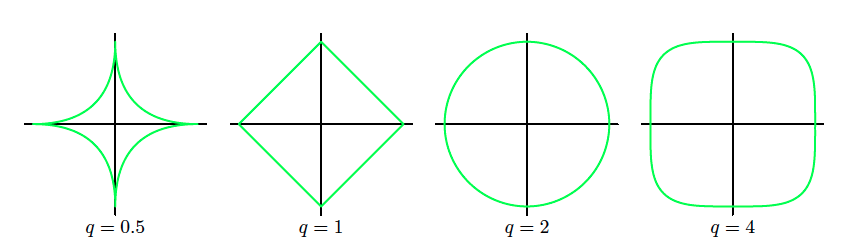
\includegraphics[scale=0.3]{images/regularization.png}
\end{center}

\end{frame}

\begin{frame}{Перцептрон: результаты}

	\begin{center}
   		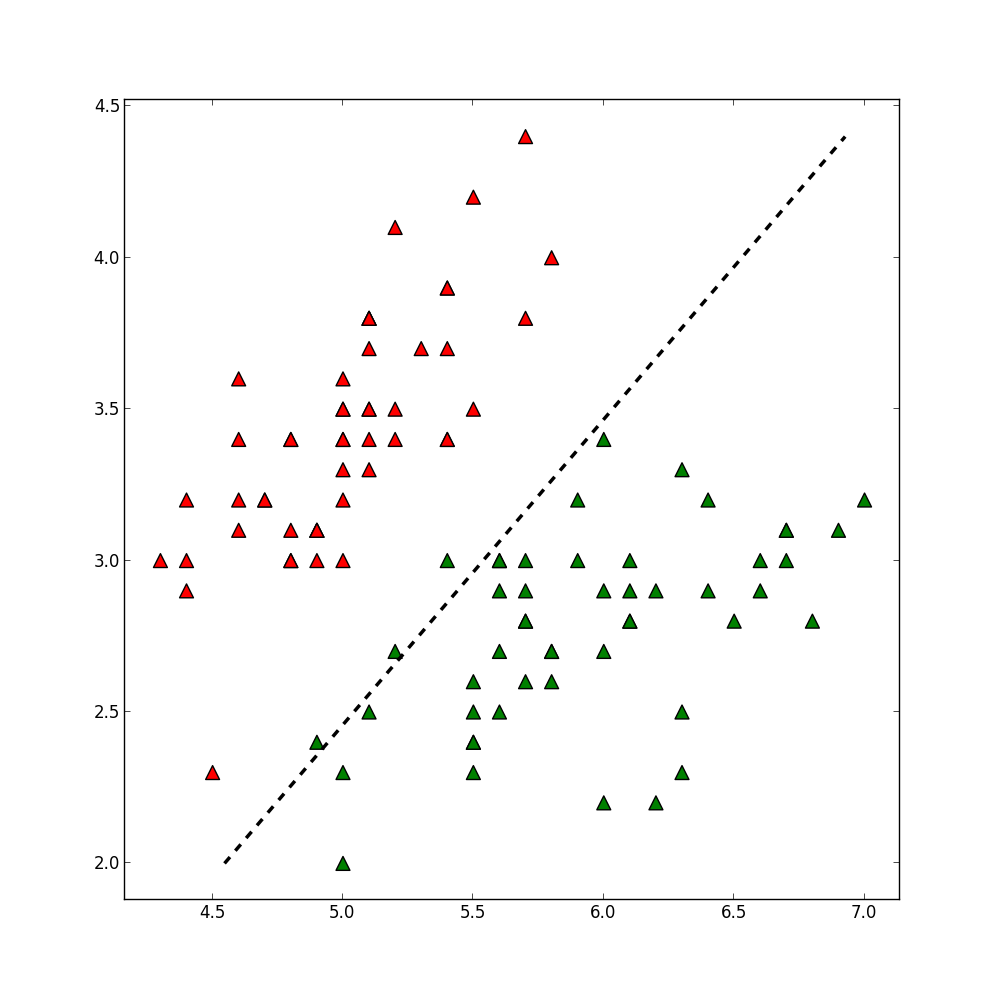
\includegraphics[scale=0.2]{images/perc01.png}\;   		
   		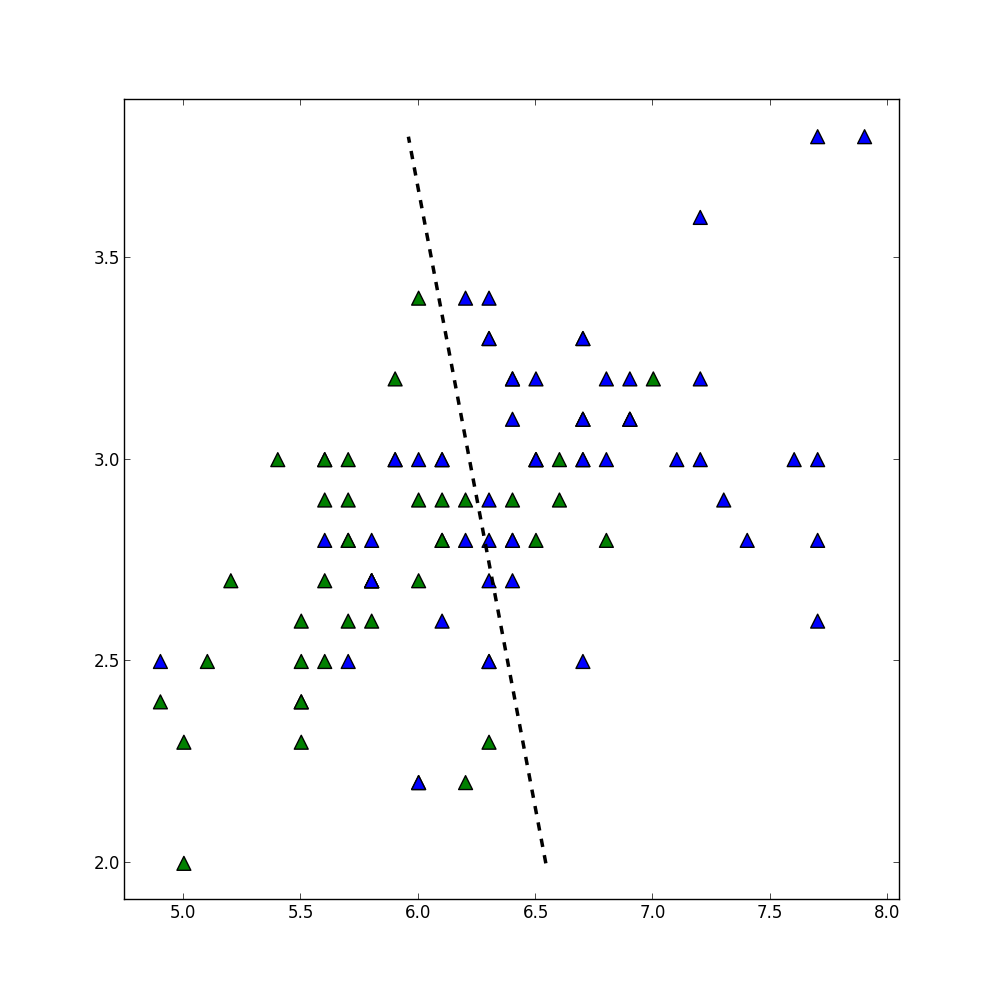
\includegraphics[scale=0.2]{images/perc12.png}
    \end{center}

\end{frame}

% ============================================== %

\section{SVM}

% ============================================== %

\begin{frame}{}

\begin{center}
\Large SVM

\vspace{1em}

\includegraphics[scale=0.5]{images/svm_logo.jpg}
\end{center}

\end{frame}

\begin{frame}{Максимальный зазор}

\begin{columns}[T]
    \begin{column}{.51\textwidth}
    Margin -- наименьшее расстояние между РП и обучающим объектом.
    \[
    d_j = \frac{|y(\mathbf{x}_j)|}{\|\mathbf{w}\|} = \frac{t_j y(\mathbf{x}_j)}{\|\mathbf{w}\|} = 
    \]    
    \[
    = \frac{t_j (\mathbf{w}^\top \phi(\mathbf{x}_j) + b)}{\|\mathbf{w}\|}
    \]
    Оптимальная РП
    \[
    \arg \max_{\mathbf{w}, b} \left[\frac{1}{\|\mathbf{w}\|} \min_j t_j (\mathbf{w}^\top \phi(\mathbf{x}_j) + b) \right]
    \]
	
    \end{column}
       
    \begin{column}{.5\textwidth}
    \vspace{-0em}
	\begin{center}
   		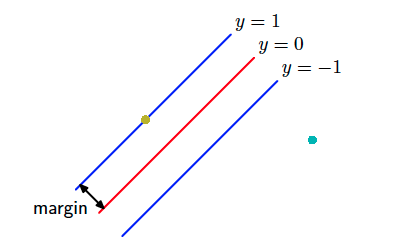
\includegraphics[scale=0.45]{images/margin.png}
    \end{center}
    \end{column}
  \end{columns}
  
\end{frame}

\begin{frame}{Задача оптимизации}

Расстояние от точки $x_j$ до РП
\[
d_j = \frac{t_j (\mathbf{w}^\top \phi(\mathbf{x}_j) + b)}{\|\mathbf{w}\|}
\]

Для точки $x_j$, лежащей на минимальном расстоянии от РП положим
\[
t_j (\mathbf{w}^\top \phi(\mathbf{x}_j) + b) = 1
\]

\begin{framed}
{\bf Задача оптимизации}
\begin{eqnarray*}
&& \frac 1 2 \|\mathbf{w}\|^2 \rightarrow \min_{\mathbf{w}, b} \\
&& \text{при условиях} \\
&& t_j (\mathbf{w}^\top \phi(\mathbf{x}_j) + b) \geq 1, \;\; \forall j \in 1,\ldots,N
\end{eqnarray*}
\end{framed}

\end{frame}

\begin{frame}{}

Метод множителей Лагранжа $\mathbf{a} = (a_1, \ldots, a_N)^\top,\;a_i \geq 0$.
\[
L(\mathbf{w}, b, \mathbf{a}) = \frac 1 2 \|\mathbf{w}\|^2 - \sum_{j=1}^N a_j [t_j (\mathbf{w}^\top \phi(\mathbf{x}_j) + b) - 1]
\]
Дифференцируем по $\mathbf{w}$ и $b$
\[
\mathbf{w} = \sum_{j=1}^N a_j t_j \phi(\mathbf{x}_j), \;\; 0 = \sum_{j=1}^N a_j t_j
\]
Подставляем $\mathbf{w}$ и $b$ в лагранжиан

\end{frame}

\begin{frame}{Сопряженная задача}

\begin{framed}
{\bf Сорпяженная задача}
\begin{eqnarray*}
&& \tilde{L}(\mathbf{a}) = \sum_{j=1}^N a_j - \frac{1}{2} \sum_{i=1}^N \sum_{j=1}^N a_i a_j t_i t_j \phi(\mathbf{x}_i)^\top \phi(\mathbf{x}_j) \rightarrow \max_{\mathbf{a}} \\
&& \text{при условиях} \\
&& a_j \geq 0, \;\; \forall j \in 1,\ldots,N \\
&& \sum_{j=1}^N a_j t_j = 0\\
\end{eqnarray*}
\end{framed}

Наблюдения
\begin{itemize}
\item $k(x_i, x_j) = \phi(\mathbf{x}_i)^\top \phi(\mathbf{x}_j)$ -- неотрицательно-определенная функция
\item лагранжиан $\tilde L(\mathbf{a})$ -- выпуклая и ограниченная сверху функция
\end{itemize}

\end{frame}

\begin{frame}{Классификация}

Функция принятия решения
\[
y(\mathbf{x}) = \mathbf{w}^\top \phi(\mathbf{x}) + b = \sum_{j=1}^N a_j t_j \phi(\mathbf{x}_j)^\top  \phi(\mathbf{x}) + b = \sum_{j=1}^N a_j t_j k(\mathbf{x}_j, \mathbf{x}) + b
\]
Условия Karush-Kuhn-Tucker
\begin{eqnarray*}
a_j &\geq& 0 \\
t_j y(\mathbf{x_j}) - 1 &\geq& 0 \\
a_j \{t_j y(\mathbf{x_j}) - 1\} &=& 0
\end{eqnarray*}
{\bf Опорным векторам} $\mathbf{x}_j \in S$ соответствуют $a_j > 0$
\[
b = \frac{1}{N_s} \sum_{i \in S} \left( t_i - \sum_{j \in S} a_j t_j k(\mathbf{x_i}, \mathbf{x_j})\right)
\]

\end{frame}

\begin{frame}{Линейно-разделимый случай}

\begin{block}{Задача}
Дана обучающая выборка

\begin{center}
\begin{tabular}{l|cc|c}
 & $x_1$ & $x_2$ & $t$ \\
 \hline
$\mathbf{x}_1$ & $1$ & $-2$ & $1$ \\
$\mathbf{x}_2$ & $1$ & $2$ & $-1$ \\
\end{tabular}
\end{center}

Найти оптимальную разделяющую плоскость, используя сопряженную задачу оптимизации

\end{block}

\end{frame}

\begin{frame}{Линейно-неразделимый случай}

\begin{center}
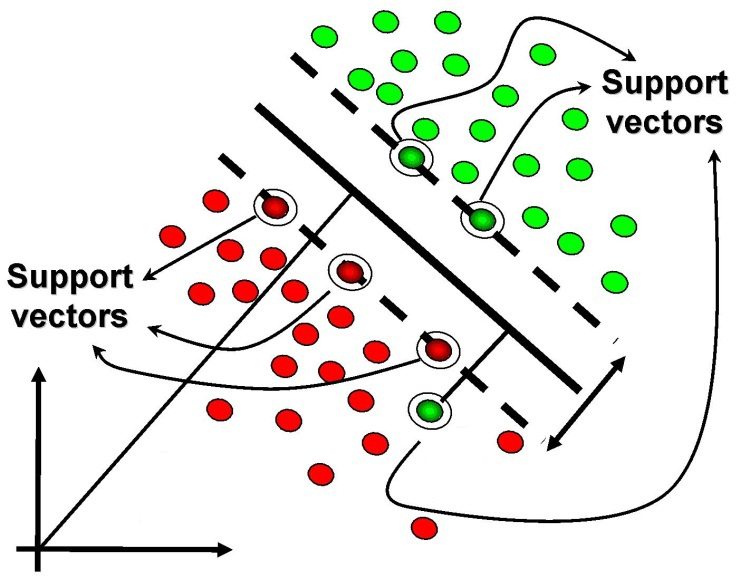
\includegraphics[scale=0.45]{images/svm.jpg}
\end{center}

\end{frame}

\begin{frame}{Смягчение ограничений}

\begin{columns}[T]
    \begin{column}{.51\textwidth}
    
    Переменные $\xi_j \geq 0$ (slacks):
    \[
    \xi_j = \begin{cases}
    0, \quad\quad\quad\quad\;\;\text{ если }y(\mathbf{x_j}) t_j \geq 1  \\
    |t_j - y(\mathbf{x}_j)|, \;\,\text{ иначе}
    \end{cases}
    \]
    Задача оптимизации
    \[
    C \sum_{j=1}^N \xi_j + \frac{1}{2}\|\mathbf{w}\|^2 \rightarrow \min_{\mathbf{w}, b}
    \]
    при условиях
    \[
		t_j y(\mathbf{x}_j) \geq 1 - \xi_j, \;\; \xi_j \geq 0
		\]

	
    \end{column}
       
    \begin{column}{.5\textwidth}
    	\vspace{-1em}
		\begin{center}
   			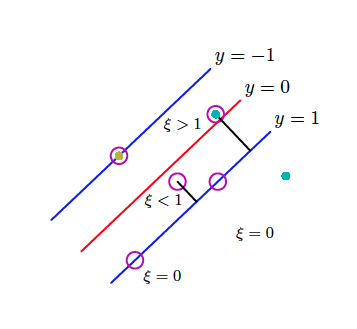
\includegraphics[scale=0.45]{images/slack.png}
    	\end{center}
	\end{column}
\end{columns}
  
\end{frame}

\begin{frame}{Сопряженная задача}

\begin{framed}
{\bf Сорпяженная задача}
\begin{eqnarray*}
&& \tilde{L}(\mathbf{a}) = \sum_{j=1}^N a_j - \frac{1}{2} \sum_{i=1}^N \sum_{j=1}^N a_i a_j t_i t_j \phi(\mathbf{x}_i)^\top \phi(\mathbf{x}_j) \rightarrow \max_{\mathbf{a}} \\
&& \text{при условиях} \\
&& 0 \leq a_j \leq C, \;\; \forall j \in 1,\ldots,N \\
&& \sum_{j=1}^N a_j t_j = 0\\
\end{eqnarray*}
\end{framed}

Наблюдения
\begin{itemize}
\item $a_j = 0$ -- правильно проклассифицированные объекты
\item $a_j = C$ -- опорные векторы внутри отступа 
\item $0 < a_j < C$ -- опорные векторы на границе
\end{itemize}

\end{frame}

\begin{frame}{Классификация}

Функция принятия решения
\[
y(\mathbf{x}) = \sum_{j=1}^N a_j t_j k(\mathbf{x}_j, \mathbf{x}) + b
\]
Константа $b$
\[
b = \frac{1}{N_\mathcal{M}} \sum_{i \in \mathcal{M}} \left( t_i - \sum_{j \in S} a_j t_j k(\mathbf{x_i}, \mathbf{x_j})\right)
\]

\end{frame}

\begin{frame}{Задача регрессии}

\begin{columns}[T]
    \begin{column}{.51\textwidth}
    
    Переменные $\xi_j \geq 0$, $\hat \xi_j \geq 0$ (slacks):
    \[
    t_j \leq y(\mathbf{x}_j) + \epsilon + \xi_n
    \]
     \[
    t_j \geq y(\mathbf{x}_j) - \epsilon - \hat \xi_n
    \]
    Задача оптимизации
    \[
    C \sum_{j=1}^N (\hat \xi_j + \xi_j) + \frac{1}{2}\|\mathbf{w}\|^2 \rightarrow \min_{\mathbf{w}, b}
    \]    
	
    \end{column}
       
    \begin{column}{.5\textwidth}
    	\vspace{0em}
		\begin{center}
   			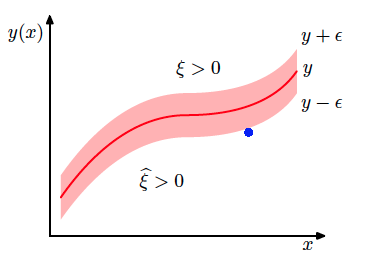
\includegraphics[scale=0.45]{images/regression.png}
    	\end{center}
	\end{column}
\end{columns}

\end{frame}

\begin{frame}{Численные методы оптимизации}

\begin{itemize}
\item Chunking (Vapnik, 1982)
\item Decomposition (Osuna, 1996)
\item Sequential Minimal Optimization (Platt, 1999)
\end{itemize}

\end{frame}

% ============================================== %

\section{Функции ядра}

% ============================================== %

\begin{frame}{}

\begin{center}
\Large Функции ядра

\vspace{1em}

\includegraphics[scale=0.5]{images/kernel_panic.jpg}
\end{center}

\end{frame}

\begin{frame}{Функции ядра}

$\phi(\mathbf{x})$ --  функция преобразования $\mathbf x$ из исходного пространства в спрямляющее пространство

\vspace{1em}
Проблема: количество признаков может быть очень велико

\vspace{1em}
\begin{block}{Идея Kernel Trick}
В процессе тренировки и применения SVM исходные векторы $\mathbf x$ используются только как аргументы в скалярном произведении $k(\mathbf x_i, \mathbf{x}_j) = \phi(\mathbf x_i)^\top \phi(\mathbf{x_j})$. Но в этом случае можно избежать вычисления $\varphi(\mathbf x)$!
\end{block}

\end{frame}

\begin{frame}{Теорема Мерсера}

\begin{alertblock}{Теорема}
Функция $k(\mathbf x, \mathbf z)$ является ядром тогда и только тогда, когда она 
\begin{itemize}
\item симметрична 
\[
k(\mathbf x, \mathbf z) = k(\mathbf z, \mathbf x)
\]
\item неотрицательно определена
\[
\int_{\mathbf x \in \mathbf X} \int_{\mathbf z \in \mathbf X} k(\mathbf x, \mathbf z) g(\mathbf x) g(\mathbf z) d\mathbf x d\mathbf z \geqslant 0, \;\; \forall g(\mathbf{x}): \mathbf{X} \rightarrow R
\]
\end{itemize}
\end{alertblock}

\begin{block}{Задача}
Пусть $\mathbf x \in R^2$, а преобразование $\phi(\mathbf{x})$
\[
\phi(\mathbf{x}) = (1, \sqrt{2} x_1, \sqrt{2} x_2, x_1^2, \sqrt{2} x_1 x_2, x_2^2).
\]
Проверить, что функция $k(\mathbf{x}, \mathbf{z}) = (1 + \mathbf x^\top \mathbf z)^2$ является функцией ядра для данного преобразования.
\end{block}

\end{frame}

\begin{frame}{Некоторые стандартные функции ядра}

\begin{itemize}
\item Линейное ядро
\[
k(\mathbf{x}, \mathbf{z}) = \mathbf{x}^\top\mathbf{z}
\]
\item Полиномиальное ядро степени $d$
\[
k(\mathbf{x}, \mathbf{z}) = (\mathbf{x}^\top\mathbf{z} + r)^d
\]
\item Radial Basis Function
\[
k(\mathbf{x}, \mathbf{z}) = e^{-\gamma |\mathbf x - \mathbf z|^2}
\]
\item Sigmoid
\[
k(\mathbf{x}, \mathbf{z}) = \tanh (\gamma \mathbf{x}^\top\mathbf{z} + r)
\]

\end{itemize}

\end{frame}

\begin{frame}{Опять ирисы}

\begin{center}
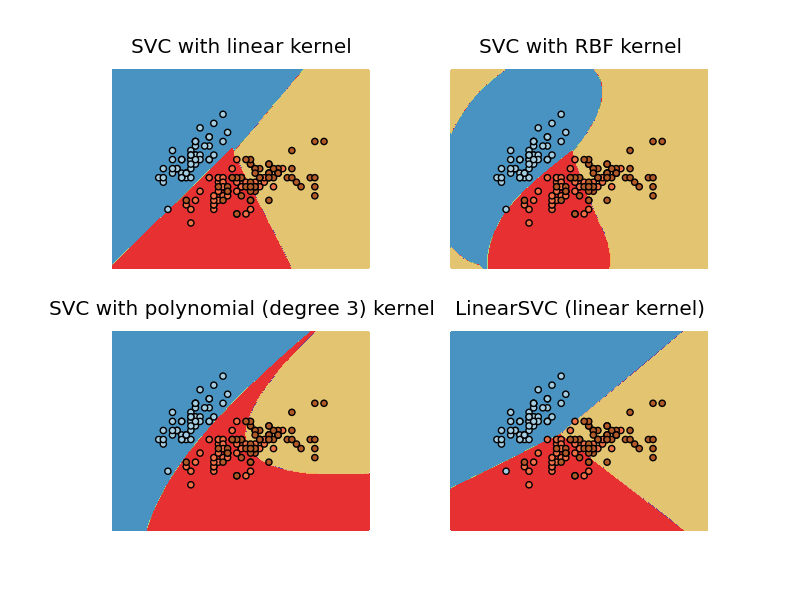
\includegraphics[scale=0.5]{images/iris.png}
\end{center}

\end{frame}

% ============================================== %

\section{SGD}

% ============================================== %

\begin{frame}{}

\begin{center}
\Large SGD

\vspace{1em}

\includegraphics[height=0.8\textheight]{images/acro.png}
\end{center}

\end{frame}

\begin{frame}{Связь с линейными моделями}

Задача оптимизации 
\[
C \sum_{j=1}^N \xi_j + \frac{1}{2} \|w\|^2 \sim \sum_{j=1}^N E(y(\mathbf{x}_j), t_j) + \lambda \|w\|^2 \rightarrow \min_{\mathbf{w}, b}
\]
Hinge loss
\[
E(y_j, t_j) = \begin{cases}
1 - y_j t_j, \text{ если } y_j t_j < 1 \\
0, \quad\quad\;\;\,\text{ иначе }
\end{cases}
\]

\end{frame}

\begin{frame}{Stochastic Gradient Descent}

Градиентный спуск
\[
\mathbf{w}_{k+1} = \mathbf{w}_k - \eta(k) \frac 1 N \sum_{n=1}^N \nabla_\mathbf{w} l(\mathbf{x_n, \mathbf{w}}, t_n)
\]
Стохастический градиентный спуск
\[
\mathbf{w}_{k+1} = \mathbf{w}_k - \eta(k) \nabla_\mathbf{w} l(\mathbf{x_k, \mathbf{w}}, t_k)
\]
Усредненный стохастический градиентный спуск $\bar{\mathbf{w}}_k = \frac 1 k \sum_{j=1}^k \mathbf{w}_j$
\[
\mathbf{w}_{k+1} = \mathbf{w}_k - \eta(k) \nabla_\mathbf{w} l(\mathbf{x_k, \mathbf{w}}, t_k), \quad \bar{\mathbf{w}}_{k+1} = \frac{k}{k+1} \bar{\mathbf{w}}_{k} + \frac{1}{k+1} \mathbf{w}_{k+1}
\]
Сходимость: $\sum_k \eta_k^2 < \infty, \;\; \sum_k \eta_k = \infty$

\end{frame}

\begin{frame}{SGD tips}

\begin{itemize}
\item Использовать SGD, когда обучение модели занимает слишком много времени
\item Перемешать тренировочную выборку
\item Следить за training error и {\bf validation error}
\item Поверять, правильно ли вычисляется градиент 
\[
Q(z, w + \delta) \approx Q(z, w) + \delta g
\]
\item Подобрать $\eta_0$ на небольшой выборке 
\[
\eta_k = \eta_0 (1 + \eta_0 \lambda k)^{-1}, \quad \lambda\text{ -- параметр регуляризации}
\] 
\end{itemize}

\end{frame}

\begin{frame}{SVM -- итоги}

\begin{itemize}
\item[+] Нелинейная разделяющая поверхность
\item[+] Глобальая оптимизация
\item[+] Разреженное решение
\item[+] Хорошая обобщающая способность
\item[-] Не поддерживает $p(C_k | \mathbf x)$
\item[-] Чувствительность к выбросам
\item[-] Нет алгоритма выбора ядра
\item[-] Медленное обучение
\end{itemize}

\end{frame}

\begin{frame}{}

\begin{center}
\Large Вопросы
\end{center}

\end{frame}

\end{document}